\documentclass[a4paper]{article}
\usepackage{ucs}
\usepackage[utf8x]{inputenc}
\usepackage{changepage}
\usepackage{graphicx}
\usepackage{amsmath}
\usepackage{gensymb}
\usepackage{amssymb}
\usepackage{enumerate}
\usepackage{tabularx}
\usepackage{lipsum}
\usepackage{amsthm}
\usepackage{thmtools}
\usepackage{xcolor}



%\documentclass[jou]{apa6}
%\usepackage[american]{babel}

%\usepackage{csquotes}
%\usepackage[style=apa,sortcites=true,sorting=nyt,backend=biber]{biblatex}
%\DeclareLanguageMapping{american}{american-apa}
%\addbibresource{bibliography.bib}


%%%%%%%%%%%%%%%%%%%%%%%%%%%%%%%%%%%%%%%%
%% Discrete Structures
%% The start of RBS stuff
%%%%%%%%%%%%%%%%%%%%%%%%%%%%%%%%%%%%%%%%

% Working internal and external links in PDF
\usepackage{hyperref}
% Extra math symbols in LaTeX
\usepackage{amsmath}
\usepackage{gensymb}
\usepackage{amssymb}
% Enumerations with (a), (b), etc.
\usepackage{enumerate}
\usepackage[framemethod=TikZ]{mdframed}
\usepackage{xcolor}

\let\OLDitemize\itemize
\renewcommand\itemize{\OLDitemize\addtolength{\itemsep}{-6pt}}

\usepackage{etoolbox}
\makeatletter
\preto{\@verbatim}{\topsep=3pt \partopsep=3pt }
\makeatother

% These sizes redefine APA for A4 paper size
\oddsidemargin 0.0in
\evensidemargin 0.0in
\textwidth 6.27in
\headheight 1.0in
\topmargin -24pt
\headheight 12pt
\headsep 12pt
\textheight 9.19in



%\title{Sample Quiz 8}
%\author{Discrete Structures, Spring 2020}
%\affiliation{RBS}

%\leftheader{Discrete Sample Quiz 8}

%\abstract

%\keywords{}

\setlength\parindent{0pt}

\begin{document}

\twocolumn


\begin{center}
{\Large 1. Mājasdarbs}\\
{\Large Bezzudumu saspiešana}
\end{center}

% https://ocw.mit.edu/courses/electrical-engineering-and-computer-science/6-441-information-theory-spring-2016/assignments/

%\begin{changemargin}{10pt}{10pt}
{\footnotesize
Vairāki uzdevumi šajā mājasdarbā iespaidojušies no MIT Open Courseware: 
\url{https://bit.ly/37Aywtf} un \url{https://bit.ly/2BdK8GA}\\
}
%\end{changemargin}

{\bf Termiņš:} 2020.gada 28.septembris, līdz vakaram (23:59:59 EEST).\\
{\bf Iesniegšanas veids:} E-studiju vide.

\vspace{10pt}
{\bf 1.uzdevums (Gabalu garumu kodējums).}\\
Aplūkojam {\em Bernulli gadījumlielumu} $X$, kam 
$$\left\{
\begin{array}{l}
P(X = 0) = \dfrac{255}{256},\\[6pt]
P(X = 1) = \dfrac{1}{256}.\\
\end{array} \right.$$
(Piemēram, tiek mesta asi\-met\-ris\-ka monēta, kam ``cipars'' 
({\em heads} jeb bits $1$) uzkrīt ar varbūtību $\frac{1}{256}$.)

Virknīti ar $n$ šī gadījumlieluma vērtībām ap\-zī\-mē ar $X^n$. 
To saspiež, izmantojot {\em Gabalu garumu ko\-dē\-ju\-mu} ({\em run-length encoding}).
Katru vieninieku kodē atsevišķi, bet 
nepārtrauktiem nuļļu gabaliem izvada tikai gabalu garumus.

{\bf Algoritma apraksts:}\\
Ievadei $X^n$ saspiesto rezultātu $f(X^n)$ iegūst,
atkārtoti izpildot šos 3 soļus, ko turpina līdzkamēr 
ievade pilnībā nolasīta.

\begin{description}
\item[1.Solis] \hfill \\
Ja ievadē pirmais bits ir ``1'', tad to nolasa un 
izvadē raksta astoņas nulles: 
$\textcolor{blue}{\mathtt{00000000}}$.
\item[2.Solis] \hfill \\
Ja ievades sākumā ir $r \leq 255$ nulles, aiz kurām seko vieninieks, 
tad visas šīs nulles nolasa un 
izvadē raksta $8$-bitu virknīti \textendash{} skaitļa $r$ bināro pierakstu.
(Tā kā nuļļu skaits $r \neq 0$, tad šajā solī nerodas izvade $\textcolor{blue}{\mathtt{00000000}}$.)
\item[3.Solis] \hfill \\
Ja ievadē ir $r > 255$ pēc kārtas esošas nulles, 
tad šajā solī nolasa tikai $255$ nulles (un izvadē raksta skaitli $255$ bināri, kā iepriekšējā punktā:
$\textcolor{blue}{\mathtt{11111111}}$). Turpina pildīt 3.soli (un izvadīt skaitļa 
$255$ kodus) līdzkamēr iestājas 1.\ vai 2.\ soļa situācija.
\end{description}

Atrast saspiešanas attiecības robežu šim kodējumam:
\begin{equation}
\label{eq1}
\lim_{n \rightarrow \infty} \frac{1}{n} E(\ell(f(X^n)).
\end{equation}
Ar $E$ apzīmējam vidējo vērtību gadījumlielumam, bet
$\ell(f(X^n))$ apzīmē saspiestās virknītes garumu.

\begin{enumerate}[(A)]
\item
Atrast (\ref{eq1}) vērtību ar precizitāti līdz $10^{-8}$.
\item 
Atrast {\em entropijas ātrumu} ({\em entropy rate}) Bernulli eksperimentu virknei:
$\lim_{n \rightarrow \infty} \frac{1}{n} H(X^n)$ jeb teo\-rē\-tis\-ko robežu, cik labi 
šo virkni var saspiest. Izteikt šo lielumu ar formulu un arī aprēķināt to 
ar precizitāti līdz $10^{-8}$
\end{enumerate}

(Šī ir parodija par 4.uzdevumu no \url{https://bit.ly/2Y6mUKa}.)


\vspace{10pt}
{\bf 2.uzdevums (Gadījuma analīze).}\\
Aplūkojam ziņojumu alfabētu ar četriem ziņojumiem: 
$S = \{ \mathtt{a}, \mathtt{b}, \mathtt{c}, \mathtt{d} \}$,
kuru varbūtības ir attiecīgi $\{1/3, 1/3, 2/9, 1/9\}$.
 
\begin{enumerate}
\item Izmantot Hafmana algoritmu, lai atrastu šim ziņojumu alfabētam optimālu bezprefiksu ko\-dē\-ju\-mu.
\item Vai ar Hafmana algoritmu var konstruēt bū\-tis\-ki citādu optimālu bezprefiksu kodējumu 
(t.i.\ tādu, kas simboliem $\mathtt{a}, \mathtt{b}, \mathtt{c}, \mathtt{d}$ 
piekārto citādus kodu garumus, nevis tikai kaut kur aizstāj
\textcolor{blue}{\tt 0} ar \textcolor{blue}{\tt 1} un otrādi). 
\item Atrast bezprefiksu kodējumu, kurš arī ir optimāls, bet nevar būt radies Hafmana algoritma rezultātā.
\end{enumerate}

(Šis ir uzdevums 2.12. no \url{https://bit.ly/2Y4PKMe}, 55.lpp.)


\vspace{10pt}
{\bf 3.uzdevums (Markova process).}\\
Pieņemsim, ka {\em Markova process} (Attēls~\ref{fig:markov-chain}) 
ir jau sasniedzis stabilu stāvokli 
(jau ir notikusi pietiekami gara nejauša staigāšana pa šo varbūtisko grafu, lai 
simbolu proporcijas un secību vairs nenoteiktu sā\-kum\-stā\-vok\-lis). 


\begin{figure}[!htb]
\center{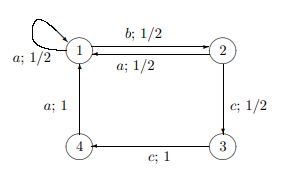
\includegraphics[width=2.6in]{markov-chain.png}}
\caption{\label{fig:markov-chain} Markova process.}
\end{figure}

Aplūkojam stabilā Markova procesa ģenerētu simbolu virkni $X^n$, kur 
$X$ pieņem vērtības no $\{\mathtt{a}, \mathtt{b}, \mathtt{c}\}$.
\begin{enumerate}[(A)]
\item Atrast saspiešanas attiecības robežu, ja simbolu virkni $X^n$ saspiež ar 
aritmētisko kodu.
\item Ar datorsimulāciju izveidot virkni $X^n$ garumā $n = 10^6$. 
Atrast saspiešanas attiecību, ja izmanto WinZip arhivatoru 
(WinZip parasti lie\-to {\em DEFLATE} algoritmu, kas ir modificēts LZ77 un 
vēl arī Hafmana kods.)
\item Atrast saspiešanas attiecības robežu ($n \rightarrow \infty$),
ja Markova virkni $X^n$ saspiež ar Hafmana kodu, 
piešķirot prefiksu kodus atsevišķiem burtiem $\{\mathtt{a}, \mathtt{b}, \mathtt{c}\}$.
\item Atrast saspiešanas attiecības robežu ($n \rightarrow \infty$),
ja Markova virkni $X^n$ saspiež ar Hafmana kodu, piešķirot prefiksu kodus 
burtu pāriem 
$$\{\mathtt{aa}, \mathtt{ab}, \ldots, \mathtt{cc}\}.$$
(Neiespējamie burtu pāri prefiksu kokā nav jāattēlo.)
\end{enumerate}

(Šī ir parodija par 2.30.uzdevumu no \url{https://bit.ly/2Y4PKMe}, 60.lpp.)



\vspace{10pt}
{\bf 5.uzdevums (I-iespēja).}\\
Teksts satur $n = 2^k$ dažādus simbolus: 
$$S = \{ s_1,s_2,\ldots,s_n \}.$$ 
To
varbūtības izkārtotas dilstošā secībā: 
$$p_1 \geq \ldots \geq p_n.$$ 

Zināms, ka ziņojumu kopai $S$
optimālu prefiksu ko\-dē\-ju\-mu veido visas 
$2^k$ vienāda garuma $k$-bitu virk\-nī\-tes. 

\begin{enumerate}[(A)]
\item Vai noteikti ir spēkā apgalvojums: Populārākā ziņojuma varbūtība 
apmierina nevienādību: 
$${\displaystyle p_1 \leq \frac{2}{2^k + 1}}?$$
\item Vai noteikti ir spēkā apgalvojums: Populārākā ziņojuma varbūtība 
nepārsniedz divu retāko ziņojumu varbūtību summu: $p_1 \leq p_{n-1} + p_{n}$?
\item Vai noteikti ir spēkā apgalvojums: Populārākā ziņojuma varbūtība 
nepārsniedz divkāršotu visretākā ziņojuma varbūtību: $p_1 \leq 2p_n$?
\end{enumerate}

(Šī ir parodija par 16.3-8.uzdevumu no {\em Introduction to Algorithms. Third Edition.} Cormen, Leiserson, Rivest, 2009.)

% https://ocw.mit.edu/courses/electrical-engineering-and-computer-science/6-450-principles-of-digital-communications-i-fall-2006/index.htm


%https://ocw.mit.edu/courses/electrical-engineering-and-computer-science/6-441-information-theory-spring-2016/assignments/MIT6_441S16_problem_set3.pdf



% https://ocw.mit.edu/courses/electrical-engineering-and-computer-science/6-050j-information-and-entropy-spring-2008/
%% Entropy related theory.

% https://ocw.mit.edu/courses/electrical-engineering-and-computer-science/6-441-information-theory-spring-2016/lecture-notes/
%% Lossy compression


% https://ocw.mit.edu/courses/electrical-engineering-and-computer-science/6-004-computation-structures-spring-2017/c1/
%% Some very easy exercises on coding.


% https://ocw.mit.edu/courses/electrical-engineering-and-computer-science/6-02-introduction-to-eecs-ii-digital-communication-systems-fall-2012/lecture-slides/
%% LZW encoding and similar










\end{document}

